\section{Lossy Compression}
\label{sec:lossy}
% \TG{You should say here that you will use lossy compression and in particular
% LTC in the future.}

In this thesis, we only focus on the lossy compression method, because the
measured sensor data intrinsically involves noise and measurement errors, which
can be treated as a configurable tolerance for a lossy compression algorithm.
Meanwhile, we sometimes prefer to sacrifice certain accuracy of reconstructed
data for a better compression ratio. In our case, Neblina has limited memory,
and in order to save more energy, we prefer a compression method with low
computational complexity so that the energy cost of the compression process is
not high. \acrshort{ltc} takes O($n$) time and O(1) space for compressing $n$
data points~\cite{schoellhammer2004lightweight}. Its good compression ratio and
very little energy cost fully meet our needs. So we will mainly discuss
\acrshort{ltc} in Chapter~\ref{chap:ltc-extension} and
Chapter~\ref{chap:expsAndResults}. 
\subsection{Lightweight Temporal Compression Algorithm}
\label{sec:ltc}

The \acrfull{ltc}~\cite{schoellhammer2004lightweight}
algorithm approximates the data stream by a piece-wise linear function of time,
with an error bounded by parameter~$\epsilon$.

The \acrshort{ltc} algorithm maintains two lines, the \emph{high line}, and the
\emph{low line} defined by (1) the latest transmitted point and (2) the
\emph{high point} (high line) and the \emph{low point} (low line). When a point
($t_i$, $x_i$) is received, the high line is updated as follows: if
$x_i+\epsilon$ is below the high line then the high line is updated to the line
defined by the last transmitted point and ($t_i$, $x_i+\epsilon$); otherwise,
the high line is not updated. Likewise, the low line is updated from
$x_i-\epsilon$. Therefore, any line located between the high line and the low
line approximates the data points received since the last transmitted point with
an error bounded by $\epsilon$~\cite{schoellhammer2004lightweight}. We assume
that the points on the high line are $(t_i, hp_i)$, and the points on low line
are $(t_i, lp_i)$, where $hp_i$ and $lp_i$ are the value of high line and low
line at corresponding time $t_i$.
The point $(t_{i-1}, \frac{hp_{(i-1)}+lp_{(i-1)}}{2})$ shall be transmitted if
the received point meets the condition:
$x_i+\epsilon < lp_{i}$ or $x_i-\epsilon > hp_{i}$. A reproduced example is
presented in Figure~\ref{fig:ltc-review}. From Figure~\ref{fig:ltc-review-b},
high line and low line is created and updated when we receive point at time
$t_2$ and $t_3$, but the condition $x_4+\epsilon < lp_{4}$ is met when point
$(t_4, x_4)$ come and we transmit point $(t_3, \frac{hp_{3}+lp_{3}}{2})$.
% \TG{There's no high line or low line in Figure 3. The labels on Figure 3 don't
% have the same size, it looks very sketchy.}

\begin{figure}
    \centering
    \begin{subfigure}{\columnwidth}
        \centering
        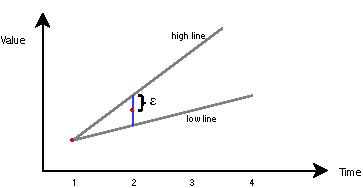
\includegraphics[height=6.2cm, width=.8\columnwidth]{figures/LTC-a.pdf}
        \caption{Create \emph{high line} and \emph{low line}}
        \label{fig:ltc-review-a}
    \end{subfigure}
    \centering
    \begin{subfigure}{\columnwidth}
        \centering
        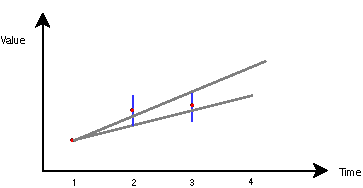
\includegraphics[height=6.2cm, width=.8\columnwidth]{figures/LTC-b.pdf}
        \caption{Update \emph{high line} and \emph{low line}}
        \label{fig:ltc-review-b}
    \end{subfigure}
    \centering
    \begin{subfigure}{\columnwidth}
        \centering
        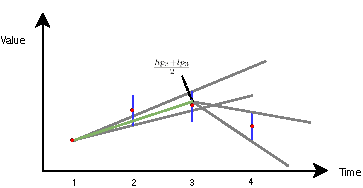
\includegraphics[height=6.2cm, width=.8\columnwidth]{figures/LTC-c.pdf}
        \caption{Transmit data point}
        \label{fig:ltc-review-c}
    \end{subfigure}
    \caption{Lightweight temporal compression example}
    \label{fig:ltc-review}
\end{figure}



\subsection{Piece-wise Linear Approximation
with Minimum number of Line Segments Algorithm}

Similar to \acrshort{ltc}, \acrfull{plamlis}~\cite{liu2007energy} represents the
original stream through a sequence of line segments. The main idea of this
algorithm is to represent the stream data over a time window using a minimum
number of segments so that the amount of data transferred is reduced.
\acrshort{plamlis} gives a greedy algorithm solution. Assume the input stream
data points $X=\{x_1, ..., x_W\}$ are received over a time window of size $W$.
Firstly, for each data points $x_i$, $i \in \{1, ..., W\}$, a longest segment
$S_{i}$ from point $x_i$ to point $x_j$ ($j>i$) is built within the error bound.
Thereby for the data points in the window, a sequence of longest segments $S =
{S_1, ..., S_W}$ is obtained. Secondly, to pick the minimum number of subsets of
S for representing original stream $X$, a greedy algorithm is used to select the
segment $S_k$ ($k \in \llbracket1, W\rrbracket$) which covers the largest number
of data points $x_i$ in $X$ at each time, then remove it from $S$ and add it
into a \texttt{result sequence} until all data points in $X$ are
covered~\cite{liu2007energy}. The result sequence is the result of
compression~\cite{zordan2012compress, zordan2014performance}.


\subsection{Enhanced Piece-wise Linear Approximation with Minimum number of Line
Segments Algorithm}

\acrfull{e-plamlis}~\cite{pham2008enhance} solves the problem ``to represent
stream data over a time window through using minimum number of segments" with a
top-down recursive segmentation algorithm which has a smaller computational cost
than \acrshort{plamlis}~\cite{pham2008enhance, zordan2014performance}. Assume
$W$ data points $x_i$ in the time window, the segment $S_{(1, W)}$ with end
points $x_1$ and $x_W$ is created, then checking whether the maximum error is
within error tolerance $\epsilon$ determines to stop the recursion or not. If
the maximum error is bigger than $\epsilon$, the segment is split into two
shorter segments $S_{(1, k)}$ and $S_{(k, W)}$ in data point $x_k$, $1<k<W$.
This procedure is applied recursively on each segment until the maximum error of
all segments is within the error tolerance~\cite{pham2008enhance,
zordan2014performance}.

\subsection{Polynomial Regression}
\label{sec:polynomial}

Different from piece-wise linear approximations, Polynomial
Regression~\cite{zordan2014performance} gives a higher order $p \geqslant1$
approximation by using standard regression methods based on least squares
fitting~\cite{phillips2003interpolation}. The approximation is a sequence of
curves (order = $p$) rather than linear segments. The algorithm starts with
collecting $p+1$ samples $\{x_1, ..., x_{p+1} \}$ to obtain the coefficients of
first $p$-order polynomial function. Upon receiving one sample $x_{p+1+i}$ at
each time, where $x_{p+1+i}$ indicates the $(p+1+i)_{th}$ sample ($i>0$) in this
approximation cycle, the best-fitting polynomial coefficients are re-computed
with $\{ x_1, ..., x_{p+1+i}\}$ and the algorithm checks whether the new
polynomial approximates the data points within the desired error tolerance. If
not, the coefficients of the previous regression are transmitted and a new
approximation starts at the current sample~\cite{zordan2014performance}.

During the compression process, all the points between transmissions need to be
kept in memory, and the least squares fitting required larger computational cost
than piece-wise linear approximations. However, polynomial regression gives
better performance in terms of \acrfull{rmse} between reconstructed data and
original data. It means that the result from the regression method is closer to
original data than result from the piece-wise linear approximation
method~\cite{zordan2014performance}.

% \begin{algorithm}
% \begin{algorithmic}[1]
% \Input
%     \Desc{$\chi$}{Received data stream}
%     \Desc{$\epsilon$}{Error bound}
%     \Desc{$p$}{The order of polynomial function}
% \EndInput
% \Output
%     \Desc{tr}{Transmitted coefficients}
% \EndOutput

% \State $S$ = $\O$
% \State $k$=1; $j$=0
% \While{True}
%     \State $S = S \cup \chi$
%     \If{$i \geqslant p+1$}
%         \State j += 1
%         \State $M_j^k$ = model($S$, $p$)    \Comment{Compute coefficients}
%         \ForAll{$x_i \in S$ and $\hat{x}_i \in$ predict($M_j^k$)}   \Comment{Check if error bound is met}
%             \If{$|\hat{x}_i - x_i| > \epsilon$}
%                 \State tr = $M_{j-1}^k$ \Comment{Transmit coefficients}
%                 \State k += 1; j = 0
%                 \State $S$ = $\chi$
%             \EndIf
%         \EndFor
%     \EndIf
% \EndWhile
% \end{algorithmic}
% \caption{Polynomial Regression Algorithm}
% \label{algo:polynomial}
% \end{algorithm}

\subsection{Adaptive Auto-Regression Moving-Average technique}


\acrfull{a-arma}~\cite{lu2010optimized} is an improved version of
\acrfull{arma}. \acrshort{arma} model is formed by combining \acrshort{ar} and
\acrshort{ma} model, and it is usually used as a tool to predict future values
over time series data~\cite{chatfield2016analysis}. The \acrshort{arma} model
\texttt{ARMA($p$, $q$)} contains $p$ \acrshort{ar} terms and $q$ \acrshort{ma}
terms. It is defined as:
\begin{equation}
X_t = \sum_{i=1}^{p}a_{i}X_{t-i} + Z_t + \sum_{i=1}^{q}\beta_{i}Z_{t-i}
\end{equation}
\noindent The equation is reproduced from~\cite{chatfield2016analysis}.
$a_1, ..., a_p$ and $\beta_1, ..., \beta_q$ are parameters of \acrshort{ar}
model and \acrshort{ma} model respectively, $Z_{t-q}, ...,Z_{t}$ are white noise
(is usually understood as residuals of the previous forecasts, $Z_t = X_t -
X_{t-1}$)~\cite{chatfield2016analysis}.

Similar to the \acrshort{arma} model, \acrshort{a-arma} is also composed of two
terms, \texttt{\acrshort{ar}} term and \texttt{\acrshort{ma}} term, respectively
predicting data value using $p$($q$) prior values or errors. To deal with the
limit of computational complexity, \acrshort{a-arma} adopts low-order
\acrshort{arma} with sliding window model~\cite{lu2010optimized}. The main idea
of \acrshort{a-arma} is maintaining and updating a \acrshort{arma} model in
memory based on sliding window.

Let's assume $W$ is a sliding window with $W$ window size, $th_{err}$ is the
minimum error tolerance on \acrfull{rmse} and $S$ means the length of each
movement of sliding window. The adapted algorithm of \acrshort{a-arma} is given
in Algorithm~\ref{algo:A-ARMA}. $model_{(p, q)}$ is the parameters of ARMA($p$,
$q$) model, obtained through function \texttt{build\_ARMA()}. Function
\texttt{go\_forward()} makes the sliding window $W$ to move $S$ length (read $S$
data samples), and function \texttt{tail($S$)} returns $S$ samples at the end of
the window. \acrshort{rmse} is calculates by function \texttt{compute\_error()}.

The first $W$ data points are used to initialize the \acrshort{arma} model, and
to compare the \acrshort{rmse} between the original and predicted subsequent $S$
data by moving sliding window $S$ length each time. If the RMSE is larger than
$th_{err}$, the saved \acrshort{arma} model is remodeled with the current
samples in sliding window~\cite{lu2010optimized}. In the decompression process,
the stream data are predicted based on the parameters transmitted.

\begin{algorithm}
\begin{algorithmic}[1]
\Input
    \Desc{$stream$}{$\quad \quad \quad $Data stream received}
    \Desc{$W$}{$\quad \quad \quad $Sliding window}
    \Desc{$th_{err}$}{$\quad \quad $Threshold of error tolerance on root-mean-square error}
    \Desc{$S$}{$\quad \quad \quad $Length of sliding window move}
    \Desc{$p$}{$\quad \quad \quad $Order of AR term}
    \Desc{$q$}{$\quad \quad \quad $Order of MA term}
\EndInput
\Output
    \Desc{$model_{(p, q)}$}{$\quad \quad \quad $Parameters of ARMA($p$, $q$) model}
\EndOutput

\State Read stream till $W$ is full \Comment{Get first $W$ data from $stream$}
\State $model_{(p, q)}$ = build\_ARMA($W$.samples, $p$, $q$)  \Comment{Build ARMA model}
\While{$stream$ is not empty}
    \State $W$.go\_forward($S$) \Comment{Moving sliding window forward $S$ length}
    \State $samples$ = $W$.tail($S$)
    \State $RMSE$ = compute\_error($samples$,  $model_{(p, q)}$.predict())
    \If{$RMSE > th_{err}$}
        \State $model_{(p, q)}$ = build\_ARMA($W$.samples, $p$, $q$)
        \State \Return $model_{(p, q)}$
    \Else
        \State \Return null \Comment{No transmitted data, model does not change}
    \EndIf
\EndWhile
\end{algorithmic}
\caption{\acrshort{a-arma} algorithm, adapted from~\cite{lu2010optimized}}
\label{algo:A-ARMA}
\end{algorithm}

\subsection{Modified Adaptive Auto-Regression}

\acrfull{ma-ar} is a modified version of \acrshort{a-arma}, proposed by Zordan
et al.~\cite{zordan2012compress}. In the \acrshort{a-arma} algorithm, the
\acrshort{arma} model is built or updated over fixed window of $W$ samples. It
might cause bad performance to predict next $S$ samples with the trained
\acrshort{arma} model over a fixed window, especially in highly noisy
environments~\cite{zordan2012compress}. Assuming the prediction cycle means a
process to find a \acrshort{ar} model which represents as much original data as
possible within error tolerance. The \acrshort{ma-ar} algorithm uses a $p$-order
\acrshort{ar} model for each prediction cycle instead of sliding window, and
controls the absolute error on each data rather than \acrshort{rmse} of $S$
continuous data. Assume $M^{(n, i)}$ indicates the \acrshort{ar} model built
according to data $\{x_n, ..., x_{n+p-1+i} \}$, where $i>0$, and
$\hat{x}_{n+p-1+i}$ indicates the predicted data, then for each prediction
cycle, \acrshort{ma-ar} works as follows:

\begin{enumerate}
    \item Collect first $p$ samples in sensor node and send them to client side.
    \item Collect one sample $x_{n+p-1+i}$ at a time, $i > 0$, to build
    $p$-order
    AR model $M^{(n, i)}$.
    \item Predict $x_{n+p-1+j}$ where $j \in \{1, ..., i\}$ using $M^{(n, i)}$.
    \item Check whether error $ |\hat{x}_{n+p-1+j} - x_{n+p-1+j}|$ is larger
    than error tolerance $\epsilon$.
        \begin{itemize}
            \item If $|\hat{x}_{n+p-1+j} - x_{n+p-1+j}| \leqslant \epsilon$, the
            model is kept. Repeat from step 2.
            \item Else the last model $M^{(n, i-1)}$ is encoded and transmitted,
            and new predict cycle is started from $x_{n+p-1+i}$.
        \end{itemize}
\end{enumerate}
The main idea of this algorithm is continuous estimations of the \acrshort{ar}
parameters. \acrshort{ar} model is redefined only according to the last coming
sample, so the computational cost is minimized and the parameters of the model
can be computed through least squares minimization~\cite{zordan2012compress}.

% \todo{add MV in chap2, and add the figure of comparison}
\todo{add the comparison in defense slides}

\subsection{Comparison of compression algorithms}
\label{sec:comparision-lossy}
% \TG{You should start a new sub-section here, or add the next paragraph to the conclusion
% section. Also, you should refer to this comparison in your thesis defense presentation.}
In~\cite{zordan2014performance}, authors compare the performance of mentioned
compression methods. They analyzed the performance in terms of compression ratio
and energy consumption in the compression process on \acrshort{ma-ar} (p={2,
4}), Polynomial Regression (p={2, 4}), \acrshort{plamlis}, \acrshort{e-plamlis}
and \acrshort{ltc}. In the aspect of compression ratio, all the methods perform
badly with the small size of data points, but with the length of input data
increasing, the compression ratio increases until approaches an asymptotic. In
their experiment, polynomial regression gives the best compression ratio, and
\acrshort{plamlis} is the second best, next, \acrshort{ltc} and
\acrshort{e-plamlis} have the same performance when the length of data is large.
Finally, \acrshort{ma-ar} method has the worst compression ratio. In terms of
energy consumption for compression, Polynomial Regression requires the most
processing energy, \acrshort{ma-ar} and \acrshort{plamlis} also need significant
processing energy. \acrshort{ltc} uses less energy for compression, because
\acrshort{ltc} only compare the high point and low point with the data point
received, and the computational complexity of each comparison process is
constant.
